
%\documentclass[xcolor=pdftex,dvipsnames,table]{beamer}
\documentclass[xcolor=pdftex,dvipsnames,table]{beamer}

\usetheme{Amsterdam}

\usefonttheme[onlymath]{serif}
\setbeamertemplate{navigation symbols}{}
\setbeamertemplate{footline}[frame number]

%\usepackage{paralist}
%\usepackage{enumerate}
\usepackage{colortbl}
\usepackage{lmodern}
\usepackage{comment}
\usepackage{natbib}
\usepackage{graphicx}
\usepackage{pbox}
\usepackage{pifont}
\usepackage{alltt}
\usepackage{verbatim}
\usepackage{multirow}
\usepackage{xspace}
\usepackage{cases}
\usepackage{geometry}
\usepackage{verbatim}
\usepackage{tikz}
\usepackage{pgf}
\usepackage[absolute,overlay]{textpos}
\usetikzlibrary{arrows,automata,positioning}
%\usepackage[absolute,overlay]{textpos}
\usepackage[normalem]{ulem}
\usepackage{tikz-qtree}
\usepackage{pbox}

\usepackage{ucs}
\usepackage[first=1, last=6]{lcg}
\usepackage[utf8x]{inputenc}
\usepackage{rotating}
%\usepackage[all]{xy}
%\usepackage{ragged2e}
%\usepackage{pifont}

%\usepackage[all]{xy}

\usepackage{latexsym}
\usepackage{amsmath}
\usepackage{amssymb}
\usepackage{xfrac}

\usepackage{notation}
\usepackage{variables}
\usepackage{drawing}
%\usepackage{xparse}
%\usepackage{tikz}
%\usetikzlibrary{calc}
\usepackage{olddef}

\newcounter{savedenum}
\newcommand*{\saveenum}{\setcounter{savedenum}{\theenumi}}
\newcommand*{\resume}{\setcounter{enumi}{\thesavedenum}}

% declares a document
\begin{document}



	%\title{Employee's social media use}
	%\title{Social media use by employees}
	\title{Hierarchical Machine Translation}
	%\subtitle{for unsupervised language learning}

	\author{Wilker Aziz}
	\institute[UvA]{
		%\inst{1}
		Universiteit van Amsterdam\\
		\texttt{w.aziz@uva.nl}
	}

	\date{\today}
	
	% Title page
	{\setbeamertemplate{footline}{}
	\begin{frame}[plain]
		\titlepage
	\end{frame}
	}


	% Table of contents	
	%\frame[allowframebreaks]{
	{\setbeamertemplate{footline}{}
	\begin{frame}
		\frametitle{Content}
		\tableofcontents
	\end{frame}
	}



	% trick to start counting from the table of contents
	\setcounter{framenumber}{0}


	% SLIDES
	\section{Motivation}

\frame{
	\frametitle{}
	\begin{figure}
	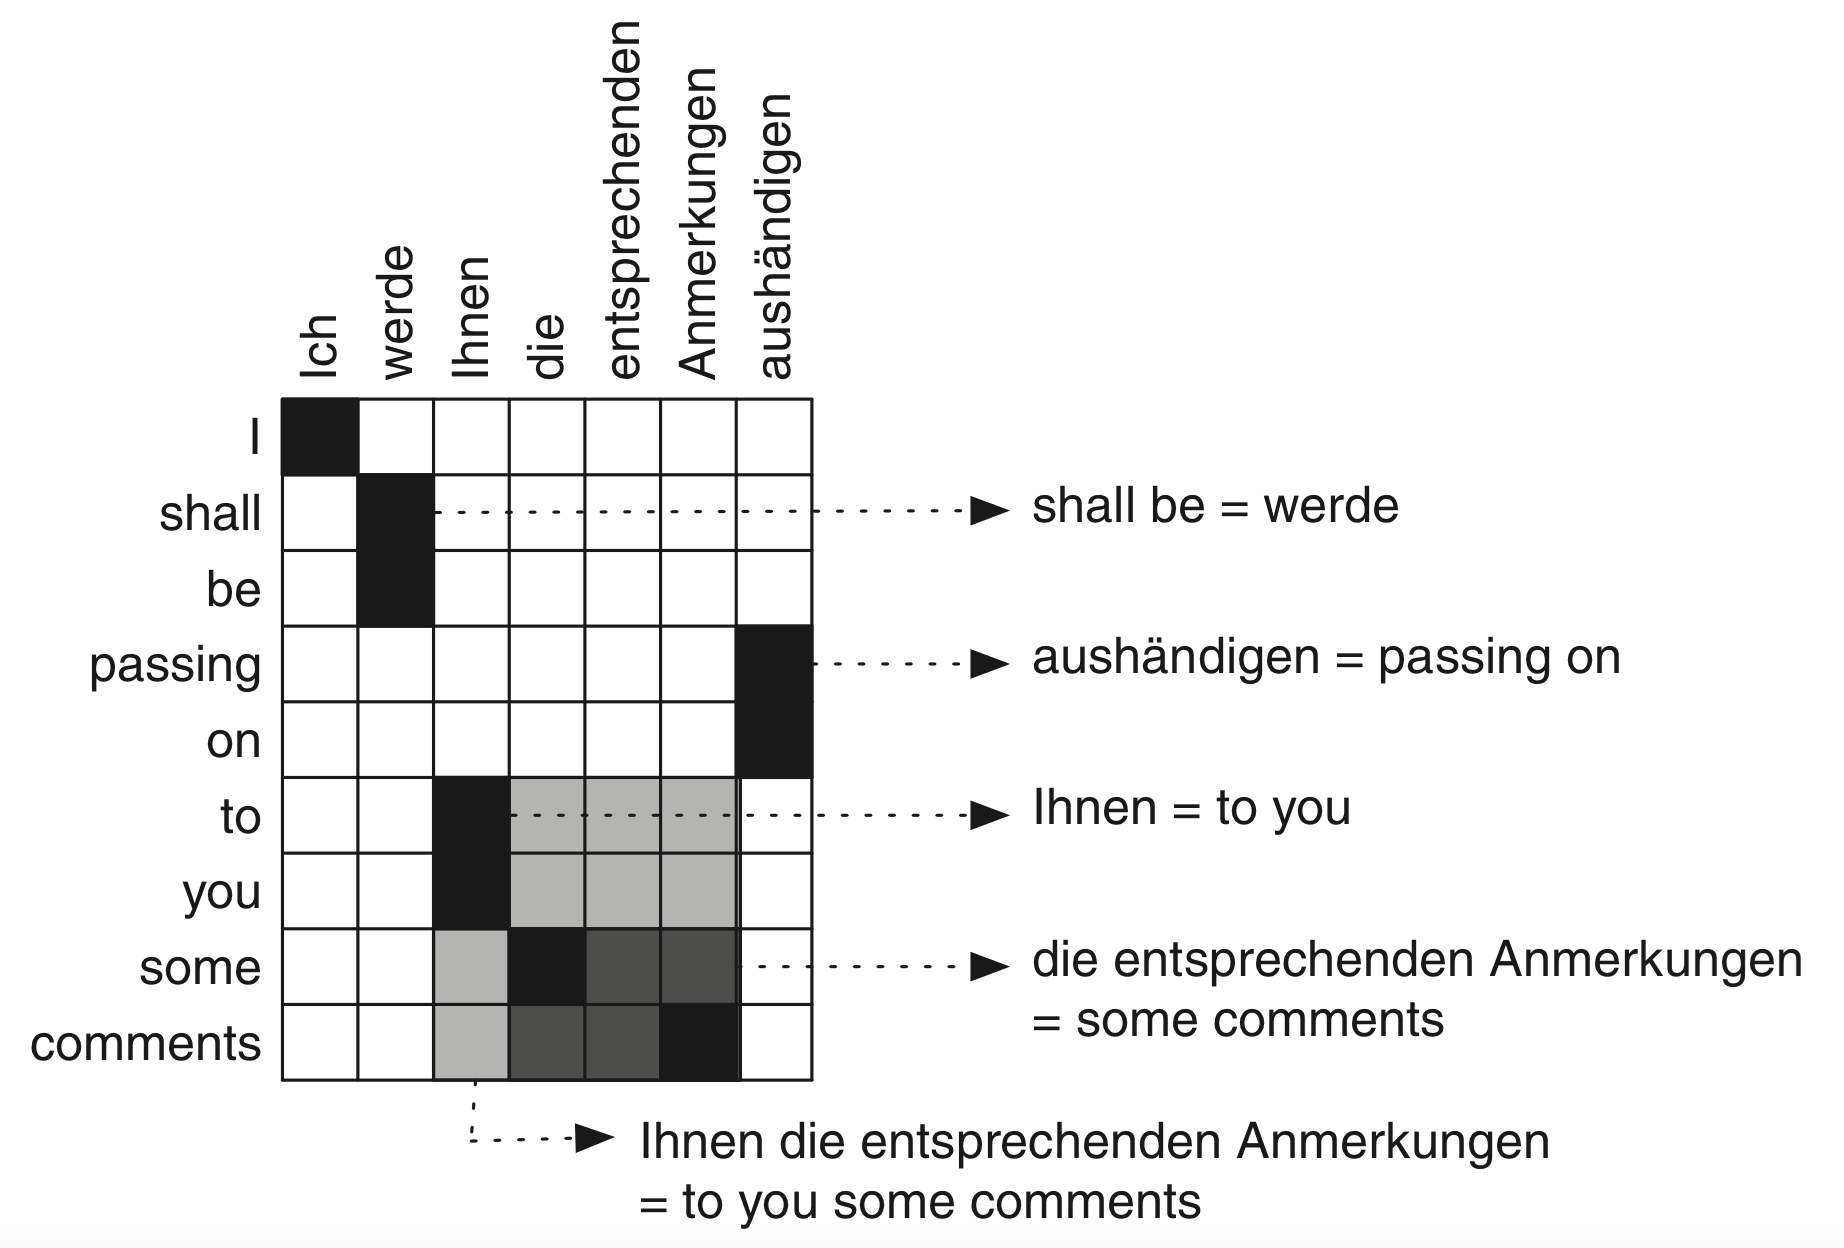
\includegraphics[scale=0.25]{img/motivation}
	\caption{\citet{Koehn:2010:SMT}}
	\end{figure}
	
	$$\ftext{werde } X \ftext{ aush\"andigen } | \etext{ shall be passing on } X $$
}


\frame{
	\frametitle{Why hierarchical structure?}
	
	Better generalisation
	\begin{itemize}
		\item compositionality
		\item reordering
	\end{itemize}
}

\frame{
	\frametitle{Why is reordering important?}
	
	Monotone translation is unrealistic
	\begin{itemize}
		\item languages differ wrt word-order\\ \pause
		e.g. different syntactic structure\\ \pause
		e.g. rich morphology \pause
	\end{itemize}

	~
	
	Reordering is arguably one of the hardest problems in MT \pause
	\begin{itemize}
		\item part of the model of translational equivalences\\
		\emph{the part that determines the space of translations}
	\end{itemize}
	
}

\frame{
	\frametitle{Key aspects}	
	
	Expressiveness
	\begin{itemize}
		\item how much can two languages differ wrt word order?
	\end{itemize}
	
	\pause
	
	Modelling
	\begin{itemize}
		\item how many parameters do we have to estimate?
	\end{itemize}

}
	%\input{expressiveness}
	
	\AtBeginSection[]
    {
    \begin{frame}<beamer>{Content}
    \tableofcontents[currentsection,currentsubsection, 
        hideothersubsections, 
        sectionstyle=show/shaded,
    ]
    \end{frame}
    }
    
    
	\section{Hierarchical models of translation}

\subsection{Hiero}

\frame{
				\frametitle{Hierarchical phrase-based - Motivation}
				Local Reordering \\
				\vspace{10pt}
				\begin{columns}
				\begin{column}{5cm}
				\only<1>{
				\begin{tabular}{|l|l|l|l|l|l|}
				\hline
				 & \vtext{J'} & \vtext{ai} & \vtext{les} & \vtext{yeux} & \vtext{noirs} \\ \hline
				 I & \celldg & & & & \\ \hline
				 have & & \celldg & & & \\ \hline
				 black & & & & & \celldg \\ \hline
				 eyes & & & \celldg & \celldg & \\ \hline
				\end{tabular}
				}
				\only<2>{
				\begin{tabular}{|l|l|l|l|l|l|}
				\hline
				 & \vtext{\cblue{J'}} & \vtext{\cblue{ai}} & \vtext{les} & \vtext{yeux} & \vtext{noirs} \\ \hline
				 \cblue{I} & \cellblue & & & & \\ \hline
				 \cblue{have} & & \celldg & & & \\ \hline
				 black & & & & & \celldg \\ \hline
				 eyes & & & \celldg & \celldg & \\ \hline
				\end{tabular}
				}
				\only<3>{
				\begin{tabular}{|l|l|l|l|l|l|}
				\hline
				 & \vtext{J'} & \vtext{ai} & \vtext{\cgreen{les}} & \vtext{\cgreen{yeux}} & \vtext{\cgreen{noirs}} \\ \hline
				 I & \celldg & & & & \\ \hline
				 have & & \celldg & & & \\ \hline
				 \cgreen{black} & & & & & \cellgreen \\ \hline
				 \cgreen{eyes} & & & \cellgreen & \cellgreen & \\ \hline
				\end{tabular}
				}
				\only<4>{
				\begin{tabular}{|l|l|l|l|l|l|}
				\hline
				 & \vtext{J'} & \vtext{\cred{ai}} & \vtext{les} & \vtext{yeux} & \vtext{\cred{noirs}} \\ \hline
				 I & \celldg & & & & \\ \hline
				 \cred{have} & & \cellr & & & \\ \hline
				 \cred{black} & & & & & \cellr \\ \hline
				 eyes & & & \celldg & \celldg & \\ \hline
				\end{tabular}
				}
				\end{column}
				\begin{column}{6cm}
					\begin{small}
					\begin{itemize}
						\item<2> Monotone\\
						\cred{J'}\indice{1} \cblue{ai}\indice{2} $\rightarrow$ \cred{I}\indice{1} \cblue{have}\indice{2}
						\item<3> Swap\\
						\cred{les yeux}\indice{4} \cblue{noirs}\indice{5} $\rightarrow$ \cblue{black}\indice{3} \cred{eyes}\indice{4}
						\item<4> Discontinuous\\
						\cred{ai}\indice{2} $X$\indice{3-4} \cblue{noirs}\indice{5} $\rightarrow$ \cred{have}\indice{2} \cblue{black}\indice{3} $X$\indice{4}
					\end{itemize}
					\end{small}
				\end{column}

				\end{columns}
			}
			\frame{
				\frametitle{Hierarchical phrase-based - Motivation}
				Discontiguous Phrases \\
				\vspace{10pt}
				\begin{columns}
				\begin{column}{5cm}
				\only<1>{
				\begin{tabular}{|l|l|l|l|l|}
				\hline
				 & \vtext{Je} & \vtext{ne} & \vtext{vais} & \vtext{pas} \\ \hline
				 I & \celldg & & & \\ \hline
				 do & & \celldg & & \celldg \\ \hline
				 not & & \celldg & & \celldg \\ \hline
				 go & & & \celldg &  \\ \hline
				\end{tabular}
				}
				\only<2>{
				\begin{tabular}{|l|l|l|l|l|}
				\hline
				 & \vtext{Je} & \vtext{\cblue{ne}} & \vtext{\cgreen{vais}} & \vtext{\cblue{pas}} \\ \hline
				 I & \celldg & & & \\ \hline
				 \cblue{do} & & \cellblue & \cellg & \cellblue \\ \hline
				 \cgreen{not} & & \cellblue & \cellg & \cellblue \\ \hline
				 \cblue{go} & & \cellg & \cellgreen & \cellg \\ \hline
				\end{tabular}
				}
				
				\end{column}
				\begin{column}{6cm}
					\begin{small}
					\begin{itemize}
						\item<2> Gappy phrase\\
						\cblue{ne} \cgreen{vais} \cblue{pas} $\rightarrow$ \cblue{do not} \cgreen{go}\\
						\cblue{ne} $X$\indice{vais} \cblue{pas} $\rightarrow$ \cblue{do not} $X$\indice{go}\\
					\end{itemize}
					\end{small}
				\end{column}

				\end{columns}
			}
			\frame{
				\frametitle{Hierarchical phrase-based - Motivation}
				Long Distance Reordering \\
				\vspace{10pt}
				\begin{columns}
				\begin{column}{6cm}
				\begin{tiny}
				\only<1>{
				\begin{tabular}{|l|l|l|l|l|l|l|l|}
				\hline
				 &  \vtext{Ich} & \vtext{werde} & \vtext{Ihnen} & \vtext{die} & \vtext{entsprechenden} & \vtext{Anmerkungen} & \vtext{aushändigen} \\ \hline
				 I & \celldg & & & & & & \\ \hline
				 shall & & \celldg & & & & & \\ \hline
				 be & & \celldg & & & & & \\ \hline
				 passing  & & & & & & & \celldg \\ \hline
				 on & & & & & & & \celldg \\ \hline
				 to & & & \celldg & & & & \\ \hline
				 you & & & \celldg & & & & \\ \hline
				 some & & & & \celldg & & & \\ \hline
				 comments & & & & & & \celldg & \\ \hline
				\end{tabular}
				}
				\only<2>{
				\begin{tabular}{|l|l|l|l|l|l|l|l|}
				\hline
				 &  \vtext{Ich} & \vtext{werde} & \vtext{Ihnen} & \vtext{die} & \vtext{entsprechenden} & \vtext{Anmerkungen} & \vtext{\cgreen{aushändigen}} \\ \hline
				 I & \celldg & & & & & & \\ \hline
				 \cblue{shall} & & \cellblue & & & & & \\ \hline
				 \cblue{be} & & \cellblue & & & & & \\ \hline
				 \cgreen{passing}  & & & & & & & \cellgreen \\ \hline
				 \cgreen{on} & & & & & & & \cellgreen \\ \hline
				 to & & & \celldg & & & & \\ \hline
				 you & & & \celldg & & & & \\ \hline
				 some & & & & \celldg & & & \\ \hline
				 comments & & & & & & \celldg & \\ \hline
				\end{tabular}
				}
				\only<3>{
				\begin{tabular}{|l|l|l|l|l|l|l|l|}
				\hline
				 &  \vtext{Ich} & \vtext{werde} & \vtext{Ihnen} & \vtext{die} & \vtext{entsprechenden} & \vtext{Anmerkungen} & \vtext{\cgreen{aushändigen}} \\ \hline
				 I & \celldg & & & & & & \\ \hline
				 \cblue{shall} & & \cellr & \cellg & \cellg & \cellg & \cellg & \cellg \\ \hline
				 \cblue{be} & & \cellr & \cellg & \cellg & \cellg & \cellg & \cellg \\ \hline
				 \cgreen{passing}  & & \cellg & \cellg & \cellg & \cellg & \cellg & \cellr \\ \hline
				 \cgreen{on} & & \cellg & \cellg & \cellg & \cellg & \cellg & \cellr \\ \hline
				 to & & & \celldg \WX & & & & \\ \hline
				 you & & & \celldg \WX & & & & \\ \hline
				 some & & & & \celldg \WX & & & \\ \hline
				 comments & & & & & & \celldg \WX & \\ \hline
				\end{tabular}
				}
				%\only<4>{
				%\begin{tabular}{|l|l|l|l|l|l|l|l|}
				%\hline
				% &  \vtext{Ich} & \vtext{werde} & \vtext{Ihnen} & \vtext{die} & \vtext{entsprechenden} & \vtext{Anmerkungen} & \vtext{\cgreen{aushändigen}} \\ \hline
				% I & \celldg & & & & & & \\ \hline
				% \cblue{shall} & & \cellr & \cellg & \cellg & \cellg & \cellg & \cellg \\ \hline
				% \cblue{be} & & \cellr & \cellg & \cellg & \cellg & \cellg & \cellg \\ \hline
				% \cgreen{passing}  & & \cellg & \cellg & \cellg & \cellg & \cellg & \cellr \\ \hline
				% \cgreen{on} & & \cellg & \cellg & \cellg & \cellg & \cellg & \cellr \\ \hline
				% to & & \cellg & \celldg & \cellg & \cellg & \cellg & \cellg \\ \hline
				% you & & \cellg & \celldg & \cellg & \cellg & \cellg & \cellg \\ \hline
				% some & & \cellg & \cellg & \celldg & \cellg & \cellg & \cellg \\ \hline
				% comments & & \cellg & \cellg & \cellg & \cellg & \celldg & \cellg\\ \hline
				%\end{tabular}
				%}
				\only<4>{
				\begin{tabular}{|l|l|l|l|l|l|l|l|}
				\hline
				 &  \vtext{Ich} & \vtext{werde} & \vtext{Ihnen}\cellbl & \vtext{die}\cellbl & \vtext{entsprechenden}\cellbl & \vtext{Anmerkungen}\cellbl & \vtext{\cgreen{aushändigen}} \\ \hline
				 I & \celldg & & & & & & \\ \hline
				 \cblue{shall} & & \cellblue & \cellg & \cellg & \cellg & \cellg & \cellg \\ \hline
				 \cblue{be} & & \cellblue & \cellg & \cellg & \cellg & \cellg & \cellg \\ \hline
				 \cgreen{passing}  & & \cellg & \cellg & \cellg & \cellg & \cellg & \cellgreen \\ \hline
				 \cgreen{on} & & \cellg & \cellg & \cellg & \cellg & \cellg & \cellgreen \\ \hline
				 to \cellbl &  & & & & & & \\ \hline
				 you \cellbl & & & & & & & \\ \hline
				 some \cellbl & & & & & & & \\ \hline
				 comments \cellbl & & & & & & & \\ \hline
				\end{tabular}
				}

				
				\end{tiny}
				\end{column}
				\begin{column}{6cm}
					\begin{small}
					\only<2>{
					\begin{itemize}
						\item How can we extract a biphrase for \textbf{shall be passing on}?
					\end{itemize}
					}
					\only<3>{
					\begin{itemize}
						\item How can we extract a biphrase for \textbf{shall be passing on}?
						\item We cannot, we need to extract \textbf{to you some comments} along
						%\item Unless we replace all those words by a non-terminal
					\end{itemize}
					}
					\only<4>{
					\begin{itemize}
						\item How can we extract a biphrase for \textbf{shall be passing on}?
						\item We cannot, we need to extract \textbf{to you some comments} along
						\item Unless we replace all those words by a variable
					\end{itemize}
					}
					\end{small}
				\end{column}

				\end{columns}
			}
			\frame{
				\frametitle{Hierarchical phrase-based - Motivation}
				Long Distance Reordering \\
				\begin{center}			
				\only<1>{	
				\cblue{shall be} \cgreen{passing on} \cred{to you some comments} \\
				$\updownarrow$ \\
				\cblue{werde} \cred{Ihnen die entsprechenden Anmerkungen} \cgreen{aushändigen}
				}
				\only<2>{	
				\cblue{shall be} \cgreen{passing on} \xout{\cred{to you some comments}} \\
				$\updownarrow$ \\
				\cblue{werde} \xout{\cred{Ihnen die entsprechenden Anmerkungen}} \cgreen{aushändigen}
				}
				\only<3>{	
				\cblue{shall be} \cgreen{passing on} \cred{$X$} \\
				$\updownarrow$ \\
				\cblue{werde} \cred{$X$} \cgreen{aushändigen}
				}
				\end{center}
				
			}
			
			
			

\frame{
	\frametitle{Hiero}

	Extends phrase-based MT with hierarchical rules \citep{Chiang:2005:HPBSMT}
	\pause
	
	\begin{itemize}
		\item conditions on word alignment \pause
		\item heuristic rule extraction \pause
		\item heuristic scoring by relative frequency counting	 \pause
		\item log-linear model \pause
		\item SCFG decoding \pause
	\end{itemize}
	
	\pause
	
	Motivation
	\begin{itemize}
		\item long-distance reordering \pause
		\item lexicalised reordering   
	\end{itemize}
	
	
}
			
			
			\frame{
				\frametitle{Heuristic rule extraction}
				\begin{center}			
				\only<1>{	
				\cblue{shall be} \cgreen{passing on} \cgray{to you} \cred{some comments} \\
				$\updownarrow$ \\
				\cblue{werde} \cgray{Ihnen} \cred{die entsprechenden Anmerkungen} \cgreen{aushändigen}
				}
				\only<2>{	
				\cblue{shall be} \cgreen{passing on} \xout{\cgray{to you}} \cred{some comments} \\
				$\updownarrow$ \\
				\cblue{werde} \xout{\cgray{Ihnen}} \cred{die entsprechenden Anmerkungen} \cgreen{aushändigen}
				}
				\only<3>{	
				\cblue{shall be} \cgreen{passing on} \cgray{$X_1$} \cred{some comments} \\
				$\updownarrow$ \\
				\cblue{werde} \cgray{$X_1$} \cred{die entsprechenden Anmerkungen} \cgreen{aushändigen}
				}
				\only<4>{	
				\cblue{shall be} \cgreen{passing on} \cgray{$X_1$} \xout{\cred{some comments}} \\
				$\updownarrow$ \\
				\cblue{werde} \cgray{$X_1$} \xout{\cred{die entsprechenden Anmerkungen}} \cgreen{aushändigen}
				}
				\only<5>{	
				\cblue{shall be} \cgreen{passing on} \cgray{$X_1$} \cred{$X_2$} \\
				$\updownarrow$ \\
				\cblue{werde} \cgray{$X_1$} \cred{$X_2$} \cgreen{aushändigen}
				}
				\end{center}
				\only<6>{	
				\begin{small}
				$[X] \rightarrow $ \cblue{shall be} \cgreen{passing on} \cgray{$X_1$} \cred{$X_2$} 
				$|$ 
				\cblue{werde} \cgray{$X_1$} \cred{$X_2$} \cgreen{aushändigen}\\
				\vspace{5pt}
				$[X] \rightarrow $ \cblue{shall be} \cgreen{passing on} \cbrown{$X_3$} 
				$|$ 
				\cblue{werde} \cbrown{$X_3$} \cgreen{aushändigen}\\
				\vspace{5pt}
				$[X] \rightarrow $ \cgray{to you} $|$ \cgray{Ihnen}\\
				\vspace{5pt}
				$[X] \rightarrow$ \cred{some comments} $|$ \cred{die entsprechenden Anmerkungen}\\
				\vspace{5pt}
				$[X] \rightarrow$ \cgray{to you} \cred{some comments} $|$ \cgray{Ihnen} \cred{die entsprechenden Anmerkungen}\\
				\end{small}
				}			
			}
			
			\frame{
				\frametitle{Hiero - Constraints}
				Practical Limitations \citep{Chiang:2005:HPBSMT}
				\begin{itemize}
					\pause
					\item at most two nonterminal symbols
					\pause
					\item $X$ spans at least 1 and at most 15 source words
					\pause
					\item no nonterminals next to each other in the source side\\
					\pause
					\begin{center}
					\cred{les} \cblue{grandes} \cbrown{maisons} $\leftrightarrow$ \cred{the} \cblue{big} \cbrown{houses\\}
					\cred{les} \cblue{$X_1$} \cbrown{maisons} $\leftrightarrow$ \cred{the} \cblue{$X_1$} \cbrown{houses}\\
					\cred{les} \cblue{$X_1$} \cbrown{$X_2$} $\leftrightarrow$ \cred{the} \cblue{$X_1$} \cbrown{$X_2$}\\
					\cred{les} $X$ $\leftrightarrow$ \cred{the} $X$\\
					\end{center}
				\end{itemize}
				\pause
				Glue rules
				\begin{itemize}
					\item $S \ra \angbrack{S_1 X_2, S_1 X_2}$ 
				\end{itemize}
			}
			\frame{
				\frametitle{Hiero - Scoring}
				\begin{footnotesize}
				Relative frequency: assume all fragments have been ``observed''\\
				\begin{itemize}
					\pause
					\item Joint rule probatility: $p(LHS, RHS_{source},RHS_{target})$\\
					\pause
					\begin{center}
						$p(X, \text{la maison } X_1, \text{the } X_1 \text{ house})$
					\end{center}
					\pause
					\item Rule application probability: $p(RHS_{source},RHS_{target}|LHS)$\\
					\pause
					\begin{center}
						$p(\text{la maison } X_1, \text{the } X_1 \text{ house} | X)$
					\end{center}
					\pause
					\item Direct translation probability: $p(RHS_{target}|RHS_{source},LHS)$\\
					\pause
					\begin{center}
						$p(\text{the } X_1 \text{ house} |\text{la maison } X_1, X)$
					\end{center}
					\pause
					\item Noisy-channel translation probability: $p(RHS_{source}|RHS_{target},LHS)$\\
					\pause
					\begin{center}
						$p(\text{la maison } X_1 |\text{the } X_1 \text{ house}, X)$
					\end{center}
					\pause
					\item Lexical translation probability\\
					\pause
					\begin{center}
					$\prod_{t_i \in RHS_{target}} p(t_i|RHS_{source},a)$ \hspace{10pt}
					$\prod_{s_i \in RHS_{source}} p(s_i|RHS_{target},a)$\\
					\end{center}
				\end{itemize}
				\end{footnotesize}
			}
			\frame{
				\frametitle{Hiero - Model}
				Log-linear combination of features

					\pause

					\begin{center}
						$p(\mdd, \mxx) = \prod_i \phi_i(\mdd, \mxx)^{\lambda_i}$
					\end{center}
					\pause
					\begin{center}
						$\log p(\mdd, \mxx) = \sum_i \lambda_i \log \phi_i(\mdd, \mxx)$
					\end{center}
					\pause
					\begin{center}
						$\log p(\mdd, \mxx) = \sum_i \lambda_i \log \prod_{r \in \mdd} \phi_i(r, \mxx)$
					\end{center}
					\pause
					\begin{center}
						$\log p(\mdd, \mxx) = \sum_i \lambda_i \left( \sum_{r \in \mdd} \log \phi_i(r, \mxx) \right)$
					\end{center}
					\pause
					\begin{center}
						$\log p(\mdd, \mxx) = \sum_{r \in \mdd} \sum_i \lambda_i \log \phi_i(r, \mxx)$
					\end{center}

				\pause
				Linear model
				$$f(\mdd, \mxx) = \sum_i \lambda_i h_i(\mdd, \mxx) = \sum_{r\in \mdd} \pmb \lambda^\top \mathbf{h}(r, \mxx)$$
			}

\subsection{Syntactic constraints}
		\frame[plain]{
				\frametitle{Syntactic Constraints}
				Rules are learnt from the word-alignment\\
				And constrained by syntactic categories\\

				\only<1>{	
				\begin{columns}
				\begin{column}{4cm}
				\resizebox{4cm}{!} {				
				\Tree
				[.S
					[ J' ].PRP0
					[.VP0
						[ ai ].VB
						[.NP0
							[ \text{les} ].DT
							[ \text{yeux} ].NN
							[ \text{noirs} ].JJ
						]
					]
				]
				}
				\end{column}
				\begin{column}{4cm}
				\resizebox{4cm}{!} {				
				\Tree
				[.S
					[ I ].PRP
					[.VP
						[ have ].VB
						[.NP
							[ black ].JJ
							[ eyes ].NN
						]
					]
				]
				}	
				\end{column}
				\end{columns}
				\begin{columns}
				\begin{column}{4cm}
					\resizebox{4cm}{!} {
					\begin{tabular}{|l|l|l|l|l|l|}
						\hline
						& J' & ai & les & yeux & noirs \\ \hline
						I  & \celldg & & & & \\ \hline
						have  & & \celldg & & & \\ \hline
						black  & & & & & \celldg \\ \hline
						eyes  & & & \celldg & \celldg & \\ \hline
					\end{tabular}
					}
				\end{column}
				\begin{column}{7cm}
				\begin{footnotesize}			
				\begin{itemize}
					\item A context-free rule requires a single LHS
					\item A rule must be consistent with word-alignment
					\item Nonterminals in the RHS must align one-to-one
				\end{itemize}
				\end{footnotesize}
				\end{column}
				\end{columns}
				}
				\only<2>{	
				\begin{columns}
				\begin{column}{4cm}
				\resizebox{4cm}{!} {				
				\Tree
				[.S
					[ J' ].PRP0
					[.VP0
						[ ai ].VB
						[.NP0
							[ les ].DT
							[ yeux ].NN
							[ \cblue{noirs} ].{\cblue{\textbf{JJ}}}
						]
					]
				]
				}
				\end{column}
				\begin{column}{4cm}
				\resizebox{4cm}{!} {				
				\Tree
				[.S
					[ I ].PRP
					[.VP
						[ have ].VB
						[.NP
							[ \cblue{black} ].{\cblue{\textbf{JJ}}}
							[ eyes ].NN
						]
					]
				]
				}	
				\end{column}
				\end{columns}
				\begin{columns}
				\begin{column}{4cm}
					\resizebox{4cm}{!} {
					\begin{tabular}{|l|l|l|l|l|l|}
						\hline
						& J' & ai & \cblue{les} & \cblue{yeux} & \cblue{noirs} \\ \hline
						I  & \celldg & & & & \\ \hline
						have  & & \celldg & & & \\ \hline
						\cblue{black}  & & &  &  & \cellblue \\ \hline
						\cblue{eyes}  & & & \celldg & \celldg &  \\ \hline
					\end{tabular}					
					}
					
					
					\vspace{5pt}					
					\begin{footnotesize}
					\cblue{\textbf{JJ}} $\rightarrow$ \cblue{noirs} $|$ \cblue{black} \\is straightforward
					\end{footnotesize}
					
				\end{column}
				\begin{column}{7cm}	
				\begin{footnotesize}			
				\begin{itemize}
					\item A context-free rule requires a \cgreen{single LHS}
					\item A rule must be \cgreen{consistent with word-alignment}
					\item Nonterminals in the RHS must \cgreen{align one-to-one}
				\end{itemize}
				\end{footnotesize}
				\end{column}
				\end{columns}
				}
				\only<3>{	
				\begin{columns}
				\begin{column}{4cm}
				\resizebox{4cm}{!} {				
				\Tree
				[.S
					[ J' ].PRP0
					[.VP0
						[ ai ].VB
						[.NP0
							[ les ].DT
							[ yeux ].NN
							[ \textbf{noirs} ].JJ
						]
					]
				]
				}
				\end{column}
				\begin{column}{4cm}
				\resizebox{4cm}{!} {				
				\Tree
				[.S
					[ I ].PRP
					[.VP
						[ have ].VB
						[.NP
							[ \textbf{black} ].JJ
							[ eyes ].NN
						]
					]
				]
				}	
				\end{column}
				\end{columns}
				\begin{columns}
				\begin{column}{4cm}
					\resizebox{4cm}{!} {
					\begin{tabular}{|l|l|l|l|l|l|}
						\hline
						& J' & ai & les & yeux & noirs \\ \hline
						I  & \celldg & & & & \\ \hline
						have  & & \celldg & & & \\ \hline
						black  & & & & & \celldg \\ \hline
						eyes  & & & \celldg & \celldg & \\ \hline
					\end{tabular}
					}
				\end{column}
				\begin{column}{7cm}
				\begin{footnotesize}			
				\begin{itemize}
					\item A context-free rule requires a single LHS
					\item A rule must be consistent with word-alignment
					\item Nonterminals in the RHS must align one-to-one
				\end{itemize}
				\end{footnotesize}
				\end{column}
				\end{columns}
				}

				\only<4>{	
				\begin{columns}
				\begin{column}{4cm}
				\resizebox{4cm}{!} {				
				\Tree
				[.S
					[ J' ].PRP0
					[.VP0
						[ ai ].VB
						[.NP0
							[ \cblue{les} ].DT
							[ \cblue{yeux} ].{NN}
							[ \textbf{noirs} ].JJ
						]
					]
				]
				}
				\end{column}
				\begin{column}{4cm}
				\resizebox{4cm}{!} {				
				\Tree
				[.S
					[ I ].PRP
					[.VP %!{\qframesubtree}
						[ have ].VB
						[.{NP}
							[ \textbf{black} ].JJ
							[ \cblue{eyes} ].NN
						]
					]
				]
				}	
				\end{column}
				\end{columns}
				\begin{columns}
				\begin{column}{4cm}
					\resizebox{4cm}{!} {
					\begin{tabular}{|l|l|l|l|l|l|}
						\hline
						& J' & ai & les & yeux & noirs \\ \hline
						I  & \celldg & & & & \\ \hline
						have  & & \celldg & & & \\ \hline
						black  & & & & & \celldg \\ \hline
						eyes  & & & \cellblue & \cellblue & \\ \hline
					\end{tabular}					
					}
					
					\vspace{5pt}
									
					\begin{footnotesize}
					A single LHS $\rightarrow$ subtree
					\end{footnotesize}
				\end{column}
				\begin{column}{7cm}
				\begin{footnotesize}			
				\begin{itemize}
					\item A context-free rule \cred{requires a single LHS}
					\item A rule must be \cgreen{consistent with word-alignment}
					\item Nonterminals in the RHS \cred{must align one-to-one}
				\end{itemize}
				\end{footnotesize}
				\end{column}
				\end{columns}
				}				
				
				\only<5>{	
				\begin{columns}
				\begin{column}{4cm}
				\resizebox{4cm}{!} {				
				\Tree
				[.S
					[ J' ].PRP0
					[.VP0
						[ ai ].VB
						[.{\cblue{NP0}}
							[ \cblue{les} ].{\cred{DT}\indice{?}}
							[ \cblue{yeux} ].{NN\indice{2}}
							[ \textbf{noirs} ].{JJ\indice{1}}
						]
					]
				]
				}
				\end{column}
				\begin{column}{4cm}
				\resizebox{4cm}{!} {				
				\Tree
				[.S
					[ I ].PRP
					[.VP %!{\qframesubtree}
						[ have ].VB
						[.{\cblue{NP}}
							[ \textbf{black} ].{JJ\indice{1}}
							[ \cblue{eyes} ].{NN\indice{2}}
						]
					]
				]
				}	
				\end{column}
				\end{columns}
				\begin{columns}
				\begin{column}{4cm}
					\resizebox{4cm}{!} {
					\begin{tabular}{|l|l|l|l|l|l|}
						\hline
						& J' & ai & les & yeux & noirs \\ \hline
						I  & \celldg & & & & \\ \hline
						have  & & \celldg & & & \\ \hline
						black  & & & \cellg & \cellg & \celldg \\ \hline
						eyes  & & & \cellblue & \cellblue & \cellg \\ \hline
					\end{tabular}					
					}
					
					\vspace{5pt}
									
					\begin{footnotesize}
					Use \cblue{NP0/NP}
					\end{footnotesize}
				\end{column}
				\begin{column}{7cm}
				\begin{footnotesize}			
				\begin{itemize}
					\item A context-free rule \cgreen{requires a single LHS}
					\item A rule must be \cgreen{consistent with word-alignment}
					\item Nonterminals in the RHS \cred{must align one-to-one}
				\end{itemize}
				\end{footnotesize}
				\end{column}
				\end{columns}
				}	
				
				\only<6>{	
				\begin{columns}
				\begin{column}{4cm}
				\resizebox{4cm}{!} {				
				\Tree
				[.S
					[ J' ].PRP0
					[.VP0
						[ ai ].VB
						[.{\cblue{NP0}}
							[ \cblue{\textbf{les}} ].{\cblue{DT}}
							[ \cblue{\textbf{yeux}} ].{\cblue{NN}}
							[ \textbf{noirs} ].{\cblue{\textbf{JJ}}\indice{1}}
						]
					]
				]
				}
				\end{column}
				\begin{column}{4cm}
				\resizebox{4cm}{!} {				
				\Tree
				[.S
					[ I ].PRP
					[.VP %!{\qframesubtree}
						[ have ].VB
						[.{\cblue{NP}}
							[ \textbf{black} ].{\cblue{\textbf{JJ}}\indice{1}}
							[ \cblue{\textbf{eyes}} ].{\cblue{NN}}
						]
					]
				]
				}	
				\end{column}
				\end{columns}
				\begin{columns}
				\begin{column}{4cm}
					\resizebox{4cm}{!} {
					\begin{tabular}{|l|l|l|l|l|l|}
						\hline
						& J' & ai & les & yeux & noirs \\ \hline
						I  & \celldg & & & & \\ \hline
						have  & & \celldg & & & \\ \hline
						black  & & & \cellg & \cellg & \cellblue \WN{JJ} \\ \hline
						eyes  & & & \cellblue & \cellblue & \cellg \\ \hline
					\end{tabular}					
					}
					
					\vspace{5pt}
									
					\begin{footnotesize}
					NP0/NP $\rightarrow$ \\
					\hspace{5pt} $\overset{DT}{les}$ $\overset{NN}{yeux}$ JJ\indice{1} $|$ JJ\indice{1} $\overset{NN}{eyes}$ 
					\end{footnotesize}
				\end{column}
				\begin{column}{7cm}
				\begin{footnotesize}			
				\begin{itemize}
					\item A context-free rule \cgreen{requires a single LHS}
					\item A rule must be \cgreen{consistent with word-alignment}
					\item Nonterminals in the RHS \cgreen{must align one-to-one}
				\end{itemize}
				\end{footnotesize}
				\end{column}
				\end{columns}
				}
				
				\only<7>{	
				\begin{columns}
				\begin{column}{4cm}
				\resizebox{4cm}{!} {				
				\Tree
				[.S
					[ J' ].PRP0
					[.VP0
						[ ai ].VB
						[.{NP0}
							[ \textbf{les} ].{\textbf{DT}}
							[ \textbf{yeux} ].{\textbf{NN}}
							[ \textbf{noirs} ].{\textbf{JJ}}
						]
					]
				]
				}
				\end{column}
				\begin{column}{4cm}
				\resizebox{4cm}{!} {				
				\Tree
				[.S
					[ I ].PRP
					[.VP
						[ have ].VB
						[.NP
							[ \textbf{black} ].{\textbf{JJ}}
							[ \textbf{eyes} ].{\textbf{NN}}
						]
					]
				]
				}	
				\end{column}
				\end{columns}
				\begin{columns}
				\begin{column}{4cm}
					\resizebox{4cm}{!} {
					\begin{tabular}{|l|l|l|l|l|l|}
						\hline
						& J' & ai & les & yeux & noirs \\ \hline
						I  & \celldg & & & & \\ \hline
						have  & & \celldg & & & \\ \hline
						black  & & & & & \celldg \\ \hline
						eyes  & & & \celldg & \celldg & \\ \hline
					\end{tabular}
					}
				\end{column}
				\begin{column}{7cm}
				\begin{footnotesize}			
				\begin{itemize}
					\item A context-free rule requires a single LHS
					\item A rule must be consistent with word-alignment
					\item Nonterminals in the RHS must align one-to-one
				\end{itemize}
				\end{footnotesize}
				\end{column}
				\end{columns}
				}		
				
				\only<8>{	
				\begin{columns}
				\begin{column}{4cm}
				\resizebox{4cm}{!} {				
				\Tree
				[.S
					[ J' ].PRP0
					[.{\cblue{VP0}}
						[ \cblue{\textbf{ai}} ].{\cblue{VB}}
						[.{\cblue{\textbf{NP0}}\indice{3}}
							[ \textbf{les} ].{\textbf{DT}}
							[ \textbf{yeux} ].{\textbf{NN}}
							[ \textbf{noirs} ].{\textbf{JJ}}
						]
					]
				]
				}
				\end{column}
				\begin{column}{4cm}
				\resizebox{4cm}{!} {				
				\Tree
				[.S
					[ I ].PRP
					[.{\cblue{VP}}
						[ \cblue{\textbf{have}} ].{\cblue{VB}}
						[.{\cblue{\textbf{NP}}\indice{3}}
							[ \textbf{black} ].{\textbf{JJ}}
							[ \textbf{eyes} ].{\textbf{NN}}
						]
					]
				]
				}	
				\end{column}
				\end{columns}
				\begin{columns}
				\begin{column}{4cm}
					\resizebox{4cm}{!} {
					\begin{tabular}{|l|l|l|l|l|l|}
						\hline
						& J' & ai & les & yeux & noirs \\ \hline
						I  & \celldg & & & & \\ \hline
						have  & & \cellblue & \cellg & \cellg & \cellg \\ \hline
						black  & & \cellg & \cellg & \cellg & \cellblue \WN{NP} \\ \hline
						eyes  & & \cellg & \cellblue \WN{NP} & \cellblue \WN{NP} & \cellg \\ \hline
					\end{tabular}
					}
					
					\vspace{5pt}
									
					\begin{footnotesize}
					VP0/VP $\rightarrow$ \\
					\hspace{5pt} $\overset{VB}{ai}$ NP0\indice{3} $|$ $\overset{VB}{have}$ NP\indice{3} 
					\end{footnotesize}
				\end{column}
				\begin{column}{7cm}
				\begin{footnotesize}			
				\begin{itemize}
					\item A context-free rule requires a single LHS
					\item A rule must be consistent with word-alignment
					\item Nonterminals in the RHS must align one-to-one
				\end{itemize}
				\end{footnotesize}
				\end{column}
				\end{columns}
				}	
				
				\only<9>{	
				\begin{columns}
				\begin{column}{4cm}
				\resizebox{4cm}{!} {				
				\Tree
				[.S
					[ J' ].PRP0
					[.VP0
						[ \textbf{ai} ].{\textbf{VB}}
						[.{\textbf{NP0}}
							[ \textbf{les} ].{\textbf{DT}}
							[ \textbf{yeux} ].{\textbf{NN}}
							[ \textbf{noirs} ].{\textbf{JJ}}
						]
					]
				]
				}
				\end{column}
				\begin{column}{4cm}
				\resizebox{4cm}{!} {				
				\Tree
				[.S
					[ I ].PRP
					[.VP
						[ \textbf{have} ].{\textbf{VB}}
						[.{\textbf{NP}}
							[ \textbf{black} ].{\textbf{JJ}}
							[ \textbf{eyes} ].{\textbf{NN}}
						]
					]
				]
				}	
				\end{column}
				\end{columns}
				\begin{columns}
				\begin{column}{4cm}
					\resizebox{4cm}{!} {
					\begin{tabular}{|l|l|l|l|l|l|}
						\hline
						& J' & ai & les & yeux & noirs \\ \hline
						I  & \celldg & & & & \\ \hline
						have  & & \celldg & & & \\ \hline
						black  & & & & & \celldg \\ \hline
						eyes  & & & \celldg & \celldg & \\ \hline
					\end{tabular}
					}
				\end{column}
				\begin{column}{7cm}
				\begin{footnotesize}			
				\begin{itemize}
					\item A context-free rule requires a single LHS
					\item A rule must be consistent with word-alignment
					\item Nonterminals in the RHS must align one-to-one
				\end{itemize}
				\end{footnotesize}
				\end{column}
				\end{columns}
				}	
				
				\only<10>{	
				\begin{columns}
				\begin{column}{4cm}
				\resizebox{4cm}{!} {				
				\Tree
				[.S
					[ \cblue{\textbf{J'}} ].{\cblue{PRP0}}
					[.VP0
						[ \textbf{ai} ].{\textbf{VB}}
						[.{\textbf{NP0}}
							[ \textbf{les} ].{\textbf{DT}}
							[ \textbf{yeux} ].{\textbf{NN}}
							[ \textbf{noirs} ].{\textbf{JJ}}
						]
					]
				]
				}
				\end{column}
				\begin{column}{4cm}
				\resizebox{4cm}{!} {				
				\Tree
				[.S
					[ \cblue{\textbf{I}} ].{\cblue{PRP}}
					[.VP
						[ \textbf{have} ].{\textbf{VB}}
						[.{\textbf{NP}}
							[ \textbf{black} ].{\textbf{JJ}}
							[ \textbf{eyes} ].{\textbf{NN}}
						]
					]
				]
				}	
				\end{column}
				\end{columns}
				\begin{columns}
				\begin{column}{4cm}
					\resizebox{4cm}{!} {
					\begin{tabular}{|l|l|l|l|l|l|}
						\hline
						& J' & ai & les & yeux & noirs \\ \hline
						I  & \cellblue & & & & \\ \hline
						have  & & \celldg & & & \\ \hline
						black  & & & & & \celldg \\ \hline
						eyes  & & & \celldg & \celldg & \\ \hline
					\end{tabular}
					}
					
					\vspace{5pt}
									
					\begin{footnotesize}
					\cblue{PRP0/PRP} $\rightarrow$ \cblue{J'} $|$ \cblue{I}\\
					is straightforward 
					\end{footnotesize}
					
				\end{column}
				\begin{column}{7cm}
				\begin{footnotesize}			
				\begin{itemize}
					\item A context-free rule requires a single LHS
					\item A rule must be consistent with word-alignment
					\item Nonterminals in the RHS must align one-to-one
				\end{itemize}
				\end{footnotesize}
				\end{column}
				\end{columns}
				}	
				
				\only<11>{	
				\begin{columns}
				\begin{column}{4cm}
				\resizebox{4cm}{!} {				
				\Tree
				[.{\cblue{S}}
					[ \textbf{J'} ].{\cblue{\textbf{PRP0}}\indice{4}}
					[.{\cblue{\textbf{VP0}}\indice{5}}
						[ \textbf{ai} ].{\textbf{VB}}
						[.{\textbf{NP0}}
							[ \textbf{les} ].{\textbf{DT}}
							[ \textbf{yeux} ].{\textbf{NN}}
							[ \textbf{noirs} ].{\textbf{JJ}}
						]
					]
				]
				}
				\end{column}
				\begin{column}{4cm}
				\resizebox{4cm}{!} {				
				\Tree
				[.{\cblue{S}}
					[ \textbf{I} ].{\cblue{\textbf{PRP}}\indice{4}}
					[.{\cblue{\textbf{VP}}\indice{5}}
						[ \textbf{have} ].{\textbf{VB}}
						[.{\textbf{NP}}
							[ \textbf{black} ].{\textbf{JJ}}
							[ \textbf{eyes} ].{\textbf{NN}}
						]
					]
				]
				}	
				\end{column}
				\end{columns}
				\begin{columns}
				\begin{column}{4cm}
					\resizebox{4cm}{!} {
					\begin{tabular}{|l|l|l|l|l|l|}
						\hline
						& J' & ai & les & yeux & noirs \\ \hline
						I  & \cellblue \WN{PRP} & \cellg & \cellg & \cellg & \cellg \\ \hline
						have  & \cellg & \cellblue \WN{VP} & \cellg & \cellg & \cellg \\ \hline
						black  & \cellg & \cellg & \cellg & \cellg & \cellblue \WN{VP} \\ \hline
						eyes  & \cellg & \cellg & \cellblue \WN{VP} & \cellblue \WN{VP} & \cellg \\ \hline
					\end{tabular}
					}
					
					\vspace{5pt}
									
					\begin{footnotesize}
					S $\rightarrow$ PRP0\indice{4} VP\indice{5} $|$ PRP\indice{4} VP\indice{5}\\
					\end{footnotesize}
					
				\end{column}
				\begin{column}{7cm}
				\begin{footnotesize}			
				\begin{itemize}
					\item A context-free rule requires a single LHS
					\item A rule must be consistent with word-alignment
					\item Nonterminals in the RHS must align one-to-one
				\end{itemize}
				\end{footnotesize}
				\end{column}
				\end{columns}
				}				
					
			}
			\frame{
				\frametitle{Grammar}
				Grammar\\
				\vspace{10pt}
				\hspace{5pt} PRP0/PRP $\rightarrow$ J' $|$ I\\
				\vspace{10pt}
				\hspace{5pt} JJ $\rightarrow$ noirs $|$ black\\
				\vspace{10pt}
				\hspace{5pt} NP0/NP $\rightarrow$  $\overset{DT}{les}$ $\overset{NN}{yeux}$ JJ $|$ JJ\\
				\vspace{10pt}
				\hspace{5pt} VP0/VP $\rightarrow$  $\overset{VB}{ai}$ NP0 $|$ $\overset{VB}{have}$ NP\\
				\vspace{10pt}
				\hspace{5pt} S $\rightarrow$ PRP0 VP0 $|$ PRP VP\\
			}
			\frame{
				\frametitle{Syntax-based vs Hiero}	
				More constraints on rules\\
				\begin{center}
					Can we extract the discontiguous phrase \textbf{ai X noirs}?\\
				\end{center}
				\cblue{Hiero}: X $\rightarrow$ ai X\indice{1} noirs $|$ have black X\indice{1} \\
				\cred{Syntactic}: No! \\
				\only<1>{	
				\begin{columns}
				\begin{column}{5cm}
				\resizebox{3cm}{!} {				
				\Tree
				[.S
					[ I ].PRP
					[.{\cblue{VP}}
						[ \cblue{ai} ].VB
						[.NP
							[ les ].DT
							[ yeux ].NN
							[ \cblue{noirs} ].JJ
						]
					]
				]
				}
				\end{column}
				\begin{column}{5cm}
				\resizebox{3cm}{!} {				
				\Tree
				[.S
					[ I ].PRP
					[.{\cblue{VP}}
						[ \cblue{have} ].VB
						[.NP
							[ \cblue{black} ].JJ
							[ eyes ].NN
						]
					]
				]
				}	
				\end{column}
				\end{columns}
				}
				\only<2>{	
				\begin{columns}
				\begin{column}{5cm}
				\resizebox{3cm}{!} {				
				\Tree
				[.S
					[ I ].PRP
					[.{\cblue{VP}}
						[ \cblue{ai} ].VB
						[.NP
							[ \cred{les} ].{\cred{DT}}
							[ \cred{yeux} ].{\cred{NN}}
							[ \cblue{noirs} ].JJ
						]
					]
				]
				}
				\end{column}
				\begin{column}{5cm}
				\resizebox{3cm}{!} {				
				\Tree
				[.S
					[ I ].PRP
					[.{\cblue{VP}}
						[ \cblue{have} ].VB
						[.NP
							[ \cblue{black} ].JJ
							[ \cred{eyes} ].{\cred{NN}}
						]
					]
				]
				}	
				\end{column}
				\end{columns}
				}
				
			}

\section{Decoding}
			\frame{			
				\frametitle{Decoding}
				\begin{columns}
					\begin{column}{5cm}
						Phrase-based\\
						\begin{itemize}
							\item<2-> Left-to-Right
							\item<3-> Beam Search
						\end{itemize}
					\end{column}
					\begin{column}{5cm}
						Tree-based\\
						\begin{itemize}
							\item<2-> Bottom-Up
							\item<3-> Chart Parsing
						\end{itemize}
					\end{column}
				\end{columns}
			}
			\frame[plain,shrink]{			
				\frametitle{Decoding by Parsing}
				\begin{center}
					\only<1>{J' ai les yeux noirs}
					\only<2>{\cred{J'}\indice{1} ai les yeux noirs}
					\only<3>{\cred{J'}\indice{1} ai les yeux \cblue{noirs}\indice{2}}
					\only<4>{\cred{J'}\indice{1} ai \cgreen{les yeux}\indice{3} \cblue{noirs}\indice{2}}
					\only<5->{\cred{J'}\indice{1} \cbrown{ai}\indice{4} \cgreen{les yeux}\indice{3} \cblue{noirs}\indice{2}}
				\end{center}
				\vspace{5pt}
				
				\only<2>{
				\begin{columns}
					\begin{column}{6cm}
						%\resizebox{4cm}{!} {
						\Tree
						[ J'\indice{1} ].{PRP0\indice{1}}
						%}
					\end{column}
					\begin{column}{6cm}
						%\resizebox{4cm}{!} {
						\Tree
						[ I\indice{1} ].{PRP\indice{1}}
						%}
					\end{column}
				\end{columns}
				}
				
				\only<3>{
				\begin{columns}
					\begin{column}{6cm}
						%\resizebox{4cm}{!} {
						\Tree
						[ J'\indice{1} ].{PRP0\indice{1}}
						\hspace{20pt}
						\Tree
						[ noirs\indice{2} ].{JJ\indice{2}}
						%}
					\end{column}
					\begin{column}{6cm}
						%\resizebox{4cm}{!} {
						\Tree
						[ I\indice{1} ].{PRP\indice{1}}
						\hspace{20pt}
						\Tree
						[ black\indice{2} ].{JJ\indice{2}}
						%}
					\end{column}
				\end{columns}
				}
				
				\only<4>{
				\begin{columns}
					\begin{column}{6cm}
						%\resizebox{4cm}{!} {
						\Tree
						[ J'\indice{1} ].{PRP0\indice{1}}
						\hspace{10pt}
						\Tree
						[.{NP0\indice{3}}
							[ les\indice{3} ].{DT\indice{3}}
							[ yeux\indice{3} ].{NN\indice{3}}
							[ noirs\indice{2} ].{JJ\indice{2}}
						]
						
						%}
					\end{column}
					\begin{column}{6cm}
						%\resizebox{4cm}{!} {
						\Tree
						[ I\indice{1} ].{PRP\indice{1}}
						\hspace{10pt}
						\Tree
						[.{NP\indice{3}}
							[ black\indice{2} ].{JJ\indice{2}}
							[ eyes\indice{3} ].{NN\indice{3}}
						]
						%}
					\end{column}
				\end{columns}
				}
				
				\only<5>{
				\begin{columns}
					\begin{column}{6cm}
						%\resizebox{4cm}{!} {
						\Tree
						[ J'\indice{1} ].{PRP0\indice{1}}
						\hspace{5pt}
						\Tree
						[.{VP0\indice{4}}
							[ ai\indice{4} ].{VB\indice{4}}
							[.{NP0\indice{3}}
								[ les\indice{3} ].{DT\indice{3}}
								[ yeux\indice{3} ].{NN\indice{3}}
								[ noirs\indice{2} ].{JJ\indice{2}}
							]
						]						
						%}
					\end{column}
					\begin{column}{6cm}
						%\resizebox{4cm}{!} {
						\Tree
						[ I\indice{1} ].{PRP\indice{1}}
						\hspace{5pt}
						\Tree
						[.{VP\indice{4}}
							[ have\indice{4} ].{VB\indice{4}}
							[.{NP\indice{3}}
								[ black\indice{2} ].{JJ\indice{2}}
								[ eyes\indice{3} ].{NN\indice{3}}
							]
						]
						%}
					\end{column}
				\end{columns}
				}
				
				\only<6>{
				\begin{columns}
					\begin{column}{6cm}
						%\resizebox{4cm}{!} {
						\Tree
						[.{S\indice{5}}
							[ J'\indice{1} ].{PRP0\indice{1}}
							[.{VP0\indice{4}}
								[ ai\indice{4} ].{VB\indice{4}}
								[.{NP0\indice{3}}
									[ les\indice{3} ].{DT\indice{3}}
									[ yeux\indice{3} ].{NN\indice{3}}
									[ noirs\indice{2} ].{JJ\indice{2}}
								]
							]			
						]			
						%}
					\end{column}
					\begin{column}{6cm}
						%\resizebox{4cm}{!} {
						\Tree
						[.{S\indice{5}}
							[ I\indice{1} ].{PRP\indice{1}}
							[.{VP\indice{4}}
								[ have\indice{4} ].{VB\indice{4}}
								[.{NP\indice{3}}
									[ black\indice{2} ].{JJ\indice{2}}
									[ eyes\indice{3} ].{NN\indice{3}}
								]
							]
						]
						%}
					\end{column}
				\end{columns}
				}
				
				\vspace{5pt}

				\begin{columns}
					\begin{column}{6cm}
						\begin{tiny}
						\begin{enumerate}
							\item PRP0/PRP $\rightarrow$ J' $|$ I
							\item JJ $\rightarrow$ noirs $|$ black
							\item NP0/NP $\rightarrow$  $\overset{DT}{les}$ $\overset{NN}{yeux}$ JJ $|$ JJ
							\item VP0/VP $\rightarrow$  $\overset{VB}{ai}$ NP0 $|$ $\overset{VB}{have}$ NP
							\item S $\rightarrow$ PRP0 VP0 $|$ PRP VP
						\end{enumerate}
						\end{tiny}
					\end{column}
					\begin{column}{6cm}
						%\begin{footnotesize}
						\begin{center}
							\only<2>{\{\cred{I}\indice{1}\}}
							\only<3>{\{\cred{I}\indice{1},\cblue{black}\indice{2}\}}
							\only<4>{\{\cred{I}\indice{1}, \cblue{black}\indice{2} \cgreen{eyes}\indice{3}\}}
							\only<5>{\{\cred{I}\indice{1}, \cbrown{have}\indice{4} \cblue{black}\indice{2} \cgreen{eyes}\indice{3}\}}
							\only<6>{\{\cred{I}\indice{1} \cbrown{have}\indice{4} \cblue{black}\indice{2} \cgreen{eyes}\indice{3}\}}
						\end{center}
						%\end{footnotesize}
					\end{column}
				\end{columns}
				
			}

	
	
	%\section{Conclusion}

	\input{syntax}
		
	
	\frame{
	\frametitle{Conclusions and further reading}
	
	Hierarchical structure
	\begin{itemize}
		\item reasonable accounts of languages with different word-order \pause
		\begin{itemize}
			\item however, rather strict/fixed word-order (simpler morphology)
		\end{itemize}
	\end{itemize}
	
	\pause
	
	Linguistically-informed labels
	\begin{itemize}
		\item constrain hiero grammar \citep{Zollmann+2006:SAMT}
		\item tree-based grammars \citep{DeNeefe+2009:STAG}
		\item feature-rich models \citep{Chiang+2009:11k}
		\item tree transducers and EM training \citep{Galley+2006:CRST}
	\end{itemize}
	
	}
	
	
	\newcounter{finalframe}
	\setcounter{finalframe}{\value{framenumber}}
	
	
	{\setbeamertemplate{footline}{}
    \begin{frame}[plain]{Questions?}
    \end{frame}
  	}
	
	
	
\frame[plain]{
	\frametitle{Earley intersection}
	
	\begin{footnotesize}
	\begin{align*}
	\textsc{Axioms} & \\
	& \drule{}{\itembrack{S' \ra \bullet S, q, q}}{q \in I} \\
	\textsc{Goal} & \\
	& \itembrack{S' \ra S \bullet, q, r} ~ q \in I \wedge r \in F\\
	\textsc{Scan} & \\
	& \drule{\itembrack{X \ra \alpha \bullet x \beta, q, s}}{\itembrack{X \ra \alpha x \bullet \beta}}{\angbrack{s, x, r} \in E}\\
	\textsc{Predict} & \\
	& \drule{\itembrack{X \ra \alpha \bullet Y \beta, q, r}}{\itembrack{Y \ra \bullet \gamma, r, r}}{Y \ra \gamma \in R} \\
	\textsc{Complete} & \\
	& \drule{\itembrack{X \ra \alpha \bullet Y \beta, q, s}\itembrack{Y \ra \gamma \bullet, s, r}}{\itembrack{X \ra \alpha Y_{s,r} \bullet \beta, q, r}}{X \neq S'} \\
	\textsc{Accept} & \\
	& \drule{\itembrack{S' \ra \bullet S, q, q}\itembrack{S \ra \gamma \bullet, q, r}}{\itembrack{S' \ra  S_{q,r} \bullet, q, r}}{r \in F} 
	\end{align*}
	\end{footnotesize}

	
}




	\frame[allowframebreaks]{ \frametitle{References}
        \bibliographystyle{plainnat}
        \bibliography{../../bib}
	}

	

	% Trick to discount regular frames from the total of backup frames
	\setcounter{framenumber}{\value{finalframe}}
	
	
\end{document}
